\section{\texorpdfstring{Program Souběh - proměnné v RAM}{Program Soubeh - promenne v RAM}}

% =====================================================================================================================
	\begin{frame}
    \frametitle{Zadání}

		\begin{enumerate}
			\item Program spustí světelný vypočtený efekt na LED přípravku,
			\vspace{3mm}
			\item vždy svítí dvě led o po stanoveném časovém kroku běží proti sobě,
			\vspace{3mm}
			\item program využije globální proměnné v RAM = pojmenovaný paměťový prostor,
			\vspace{3mm}
			\item pro časování programu bude použita již napsaná funkce \textbf{wait}.
		\end{enumerate}
		
	\end{frame}
	
% =====================================================================================================================
	\begin{frame}
    \frametitle{Program - zakládání proměnných}
		
		\begin{center}
			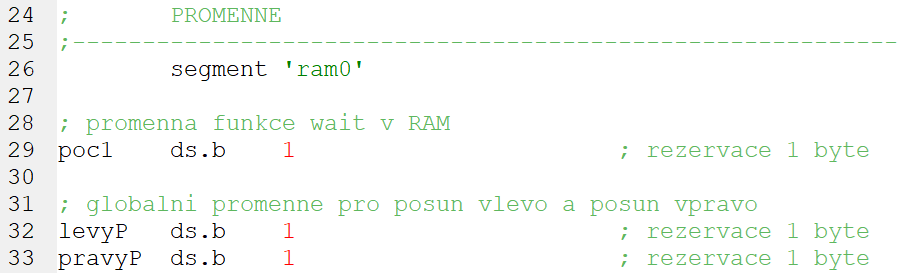
\includegraphics[width=0.80\textwidth]{fig/prg_soubeh_ram.png}
		\end{center}
		
		\begin{itemize}
			\item Direktiva \textcolor{blue}{\textbf{ds.b}} pouze přiřadí například symbolu \textbf{pravyP} hodnotu odpovídající první volné adrese v paměti RAM,
			\item lze vyhradit i více jak 1 byte, ale pak musíme k prostoru přistupovat jako k více bytové proměnné nebo jako k poli.
		\end{itemize}
		
	\end{frame}

% =====================================================================================================================
	\begin{frame}
    \frametitle{Program - hlavní smyčka}
		
		\begin{center}
			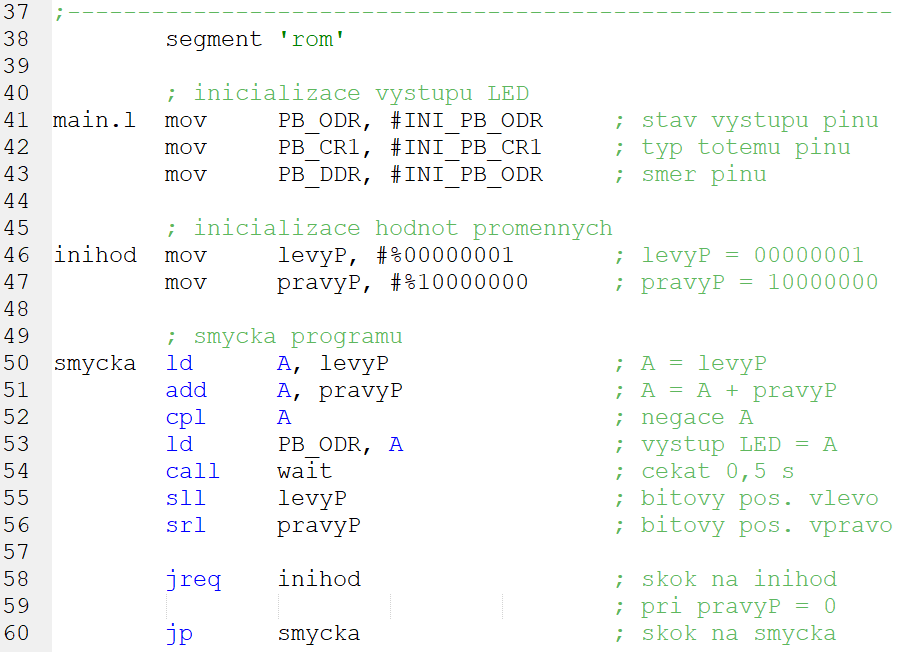
\includegraphics[width=0.80\textwidth]{fig/prg_soubeh_smycka.png}
		\end{center}
		
	\end{frame}